% Created by tikzDevice version 0.12.6 on 2026-10-30 13:02:24
% !TEX encoding = UTF-8 Unicode
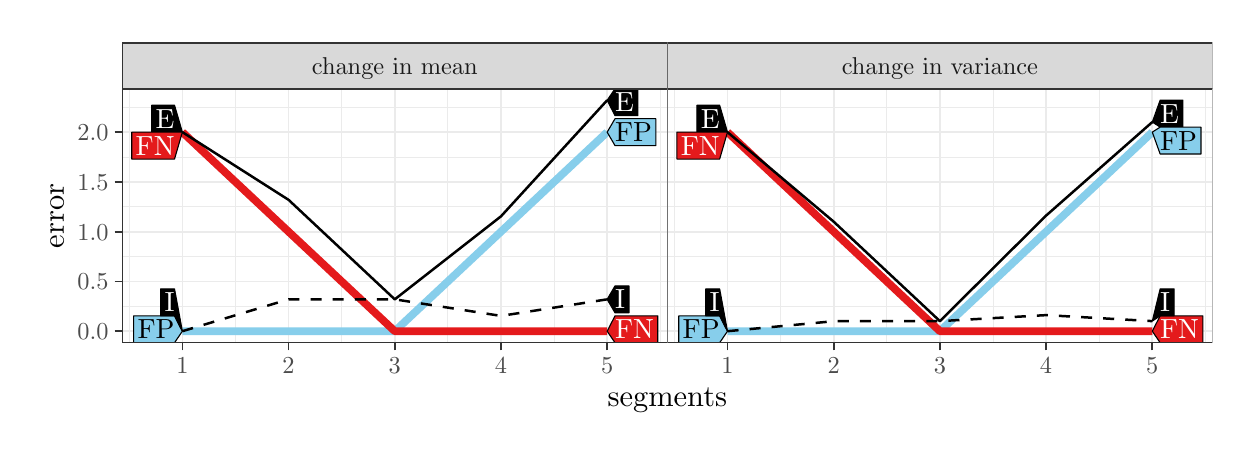
\begin{tikzpicture}[x=1pt,y=1pt]
\definecolor{fillColor}{RGB}{255,255,255}
\path[use as bounding box,fill=fillColor,fill opacity=0.00] (0,0) rectangle (433.62,144.54);
\begin{scope}
\path[clip] (  0.00,  0.00) rectangle (433.62,144.54);
\definecolor{drawColor}{RGB}{255,255,255}
\definecolor{fillColor}{RGB}{255,255,255}

\path[draw=drawColor,line width= 0.6pt,line join=round,line cap=round,fill=fillColor] (  0.00, -0.00) rectangle (433.62,144.54);
\end{scope}
\begin{scope}
\path[clip] ( 34.16, 30.69) rectangle (231.14,122.47);
\definecolor{fillColor}{RGB}{255,255,255}

\path[fill=fillColor] ( 34.16, 30.69) rectangle (231.14,122.47);
\definecolor{drawColor}{gray}{0.92}

\path[draw=drawColor,line width= 0.3pt,line join=round] ( 34.16, 43.85) --
	(231.14, 43.85);

\path[draw=drawColor,line width= 0.3pt,line join=round] ( 34.16, 61.83) --
	(231.14, 61.83);

\path[draw=drawColor,line width= 0.3pt,line join=round] ( 34.16, 79.81) --
	(231.14, 79.81);

\path[draw=drawColor,line width= 0.3pt,line join=round] ( 34.16, 97.80) --
	(231.14, 97.80);

\path[draw=drawColor,line width= 0.3pt,line join=round] ( 34.16,115.78) --
	(231.14,115.78);

\path[draw=drawColor,line width= 0.3pt,line join=round] ( 36.71, 30.69) --
	( 36.71,122.47);

\path[draw=drawColor,line width= 0.3pt,line join=round] ( 75.09, 30.69) --
	( 75.09,122.47);

\path[draw=drawColor,line width= 0.3pt,line join=round] (113.46, 30.69) --
	(113.46,122.47);

\path[draw=drawColor,line width= 0.3pt,line join=round] (151.83, 30.69) --
	(151.83,122.47);

\path[draw=drawColor,line width= 0.3pt,line join=round] (190.21, 30.69) --
	(190.21,122.47);

\path[draw=drawColor,line width= 0.3pt,line join=round] (228.58, 30.69) --
	(228.58,122.47);

\path[draw=drawColor,line width= 0.6pt,line join=round] ( 34.16, 34.86) --
	(231.14, 34.86);

\path[draw=drawColor,line width= 0.6pt,line join=round] ( 34.16, 52.84) --
	(231.14, 52.84);

\path[draw=drawColor,line width= 0.6pt,line join=round] ( 34.16, 70.82) --
	(231.14, 70.82);

\path[draw=drawColor,line width= 0.6pt,line join=round] ( 34.16, 88.81) --
	(231.14, 88.81);

\path[draw=drawColor,line width= 0.6pt,line join=round] ( 34.16,106.79) --
	(231.14,106.79);

\path[draw=drawColor,line width= 0.6pt,line join=round] ( 55.90, 30.69) --
	( 55.90,122.47);

\path[draw=drawColor,line width= 0.6pt,line join=round] ( 94.27, 30.69) --
	( 94.27,122.47);

\path[draw=drawColor,line width= 0.6pt,line join=round] (132.65, 30.69) --
	(132.65,122.47);

\path[draw=drawColor,line width= 0.6pt,line join=round] (171.02, 30.69) --
	(171.02,122.47);

\path[draw=drawColor,line width= 0.6pt,line join=round] (209.39, 30.69) --
	(209.39,122.47);
\definecolor{drawColor}{RGB}{135,206,235}

\path[draw=drawColor,line width= 2.8pt,line join=round] ( 55.90, 34.86) --
	( 94.27, 34.86) --
	(132.65, 34.86) --
	(171.02, 70.82) --
	(209.39,106.79);
\definecolor{drawColor}{RGB}{228,26,28}

\path[draw=drawColor,line width= 2.8pt,line join=round] ( 55.90,106.79) --
	( 94.27, 70.82) --
	(132.65, 34.86) --
	(171.02, 34.86) --
	(209.39, 34.86);
\definecolor{drawColor}{RGB}{0,0,0}

\path[draw=drawColor,line width= 0.9pt,line join=round] ( 55.90,106.79) --
	( 94.27, 82.33) --
	(132.65, 46.37) --
	(171.02, 76.36) --
	(209.39,118.30);

\path[draw=drawColor,line width= 0.9pt,dash pattern=on 4pt off 4pt ,line join=round] ( 55.90, 34.86) --
	( 94.27, 46.37) --
	(132.65, 46.37) --
	(171.02, 40.39) --
	(209.39, 46.37);
\end{scope}
\begin{scope}
\path[clip] ( 34.16, 30.69) rectangle (231.14,122.47);
\definecolor{drawColor}{RGB}{0,0,0}
\definecolor{fillColor}{RGB}{0,0,0}

\path[draw=drawColor,line width= 0.4pt,line join=round,line cap=round,fill=fillColor] ( 44.83,116.52) --
	( 53.06,116.52) --
	( 55.90,106.79) --
	( 53.06,106.79) --
	( 44.83,106.79) --
	cycle;
\definecolor{fillColor}{RGB}{228,26,28}

\path[draw=drawColor,line width= 0.4pt,line join=round,line cap=round,fill=fillColor] ( 37.61,106.79) --
	( 53.06,106.79) --
	( 55.90,106.79) --
	( 53.06, 97.06) --
	( 37.61, 97.06) --
	cycle;
\definecolor{fillColor}{RGB}{135,206,235}

\path[draw=drawColor,line width= 0.4pt,line join=round,line cap=round,fill=fillColor] ( 38.30, 40.42) --
	( 53.06, 40.42) --
	( 55.90, 34.86) --
	( 53.06, 30.69) --
	( 38.30, 30.69) --
	cycle;
\definecolor{fillColor}{RGB}{0,0,0}

\path[draw=drawColor,line width= 0.4pt,line join=round,line cap=round,fill=fillColor] ( 48.02, 50.15) --
	( 53.06, 50.15) --
	( 55.90, 34.86) --
	( 53.06, 40.42) --
	( 48.02, 40.42) --
	cycle;
\end{scope}
\begin{scope}
\path[clip] ( 34.16, 30.69) rectangle (231.14,122.47);
\definecolor{drawColor}{RGB}{0,0,0}
\definecolor{fillColor}{RGB}{0,0,0}

\path[draw=drawColor,line width= 0.4pt,line join=round,line cap=round,fill=fillColor] (209.39,118.30) --
	(212.24,122.47) --
	(220.47,122.47) --
	(220.47,112.74) --
	(212.24,112.74) --
	cycle;
\definecolor{fillColor}{RGB}{228,26,28}

\path[draw=drawColor,line width= 0.4pt,line join=round,line cap=round,fill=fillColor] (209.39, 34.86) --
	(212.24, 40.42) --
	(227.69, 40.42) --
	(227.69, 30.69) --
	(212.24, 30.69) --
	cycle;
\definecolor{fillColor}{RGB}{135,206,235}

\path[draw=drawColor,line width= 0.4pt,line join=round,line cap=round,fill=fillColor] (209.39,106.79) --
	(212.24,111.65) --
	(226.99,111.65) --
	(226.99,101.92) --
	(212.24,101.92) --
	cycle;
\definecolor{fillColor}{RGB}{0,0,0}

\path[draw=drawColor,line width= 0.4pt,line join=round,line cap=round,fill=fillColor] (209.39, 46.37) --
	(212.24, 51.23) --
	(217.27, 51.23) --
	(217.27, 41.50) --
	(212.24, 41.50) --
	cycle;
\definecolor{drawColor}{RGB}{255,255,255}

\node[text=drawColor,anchor=base east,inner sep=0pt, outer sep=0pt, scale=  1.00] at ( 53.06, 41.84) {I};

\node[text=drawColor,anchor=base west,inner sep=0pt, outer sep=0pt, scale=  1.00] at (212.24, 42.92) {I};
\definecolor{drawColor}{RGB}{0,0,0}

\node[text=drawColor,anchor=base east,inner sep=0pt, outer sep=0pt, scale=  1.00] at ( 53.06, 32.11) {FP};

\node[text=drawColor,anchor=base west,inner sep=0pt, outer sep=0pt, scale=  1.00] at (212.24,103.34) {FP};
\definecolor{drawColor}{RGB}{255,255,255}

\node[text=drawColor,anchor=base east,inner sep=0pt, outer sep=0pt, scale=  1.00] at ( 53.06,108.21) {E};

\node[text=drawColor,anchor=base west,inner sep=0pt, outer sep=0pt, scale=  1.00] at (212.24,114.16) {E};

\node[text=drawColor,anchor=base east,inner sep=0pt, outer sep=0pt, scale=  1.00] at ( 53.06, 98.48) {FN};

\node[text=drawColor,anchor=base west,inner sep=0pt, outer sep=0pt, scale=  1.00] at (212.24, 32.11) {FN};
\definecolor{drawColor}{gray}{0.20}

\path[draw=drawColor,line width= 0.6pt,line join=round,line cap=round] ( 34.16, 30.69) rectangle (231.14,122.47);
\end{scope}
\begin{scope}
\path[clip] (231.14, 30.69) rectangle (428.12,122.47);
\definecolor{fillColor}{RGB}{255,255,255}

\path[fill=fillColor] (231.14, 30.69) rectangle (428.12,122.47);
\definecolor{drawColor}{gray}{0.92}

\path[draw=drawColor,line width= 0.3pt,line join=round] (231.14, 43.85) --
	(428.12, 43.85);

\path[draw=drawColor,line width= 0.3pt,line join=round] (231.14, 61.83) --
	(428.12, 61.83);

\path[draw=drawColor,line width= 0.3pt,line join=round] (231.14, 79.81) --
	(428.12, 79.81);

\path[draw=drawColor,line width= 0.3pt,line join=round] (231.14, 97.80) --
	(428.12, 97.80);

\path[draw=drawColor,line width= 0.3pt,line join=round] (231.14,115.78) --
	(428.12,115.78);

\path[draw=drawColor,line width= 0.3pt,line join=round] (233.70, 30.69) --
	(233.70,122.47);

\path[draw=drawColor,line width= 0.3pt,line join=round] (272.07, 30.69) --
	(272.07,122.47);

\path[draw=drawColor,line width= 0.3pt,line join=round] (310.44, 30.69) --
	(310.44,122.47);

\path[draw=drawColor,line width= 0.3pt,line join=round] (348.82, 30.69) --
	(348.82,122.47);

\path[draw=drawColor,line width= 0.3pt,line join=round] (387.19, 30.69) --
	(387.19,122.47);

\path[draw=drawColor,line width= 0.3pt,line join=round] (425.56, 30.69) --
	(425.56,122.47);

\path[draw=drawColor,line width= 0.6pt,line join=round] (231.14, 34.86) --
	(428.12, 34.86);

\path[draw=drawColor,line width= 0.6pt,line join=round] (231.14, 52.84) --
	(428.12, 52.84);

\path[draw=drawColor,line width= 0.6pt,line join=round] (231.14, 70.82) --
	(428.12, 70.82);

\path[draw=drawColor,line width= 0.6pt,line join=round] (231.14, 88.81) --
	(428.12, 88.81);

\path[draw=drawColor,line width= 0.6pt,line join=round] (231.14,106.79) --
	(428.12,106.79);

\path[draw=drawColor,line width= 0.6pt,line join=round] (252.88, 30.69) --
	(252.88,122.47);

\path[draw=drawColor,line width= 0.6pt,line join=round] (291.26, 30.69) --
	(291.26,122.47);

\path[draw=drawColor,line width= 0.6pt,line join=round] (329.63, 30.69) --
	(329.63,122.47);

\path[draw=drawColor,line width= 0.6pt,line join=round] (368.00, 30.69) --
	(368.00,122.47);

\path[draw=drawColor,line width= 0.6pt,line join=round] (406.38, 30.69) --
	(406.38,122.47);
\definecolor{drawColor}{RGB}{135,206,235}

\path[draw=drawColor,line width= 2.8pt,line join=round] (252.88, 34.86) --
	(291.26, 34.86) --
	(329.63, 34.86) --
	(368.00, 70.82) --
	(406.38,106.79);
\definecolor{drawColor}{RGB}{228,26,28}

\path[draw=drawColor,line width= 2.8pt,line join=round] (252.88,106.79) --
	(291.26, 70.82) --
	(329.63, 34.86) --
	(368.00, 34.86) --
	(406.38, 34.86);
\definecolor{drawColor}{RGB}{0,0,0}

\path[draw=drawColor,line width= 0.9pt,line join=round] (252.88,106.79) --
	(291.26, 74.43) --
	(329.63, 38.50) --
	(368.00, 76.63) --
	(406.38,110.43);

\path[draw=drawColor,line width= 0.9pt,dash pattern=on 4pt off 4pt ,line join=round] (252.88, 34.86) --
	(291.26, 38.47) --
	(329.63, 38.50) --
	(368.00, 40.67) --
	(406.38, 38.50);
\end{scope}
\begin{scope}
\path[clip] (231.14, 30.69) rectangle (428.12,122.47);
\definecolor{drawColor}{RGB}{0,0,0}
\definecolor{fillColor}{RGB}{0,0,0}

\path[draw=drawColor,line width= 0.4pt,line join=round,line cap=round,fill=fillColor] (241.81,116.52) --
	(250.04,116.52) --
	(252.88,106.79) --
	(250.04,106.79) --
	(241.81,106.79) --
	cycle;
\definecolor{fillColor}{RGB}{228,26,28}

\path[draw=drawColor,line width= 0.4pt,line join=round,line cap=round,fill=fillColor] (234.59,106.79) --
	(250.04,106.79) --
	(252.88,106.79) --
	(250.04, 97.06) --
	(234.59, 97.06) --
	cycle;
\definecolor{fillColor}{RGB}{135,206,235}

\path[draw=drawColor,line width= 0.4pt,line join=round,line cap=round,fill=fillColor] (235.28, 40.42) --
	(250.04, 40.42) --
	(252.88, 34.86) --
	(250.04, 30.69) --
	(235.28, 30.69) --
	cycle;
\definecolor{fillColor}{RGB}{0,0,0}

\path[draw=drawColor,line width= 0.4pt,line join=round,line cap=round,fill=fillColor] (245.00, 50.15) --
	(250.04, 50.15) --
	(252.88, 34.86) --
	(250.04, 40.42) --
	(245.00, 40.42) --
	cycle;
\end{scope}
\begin{scope}
\path[clip] (231.14, 30.69) rectangle (428.12,122.47);
\definecolor{drawColor}{RGB}{0,0,0}
\definecolor{fillColor}{RGB}{0,0,0}

\path[draw=drawColor,line width= 0.4pt,line join=round,line cap=round,fill=fillColor] (406.38,110.43) --
	(409.22,118.34) --
	(417.45,118.34) --
	(417.45,108.61) --
	(409.22,108.61) --
	cycle;
\definecolor{fillColor}{RGB}{228,26,28}

\path[draw=drawColor,line width= 0.4pt,line join=round,line cap=round,fill=fillColor] (406.38, 34.86) --
	(409.22, 40.42) --
	(424.67, 40.42) --
	(424.67, 30.69) --
	(409.22, 30.69) --
	cycle;
\definecolor{fillColor}{RGB}{135,206,235}

\path[draw=drawColor,line width= 0.4pt,line join=round,line cap=round,fill=fillColor] (406.38,106.79) --
	(409.22,108.61) --
	(423.97,108.61) --
	(423.97, 98.88) --
	(409.22, 98.88) --
	cycle;
\definecolor{fillColor}{RGB}{0,0,0}

\path[draw=drawColor,line width= 0.4pt,line join=round,line cap=round,fill=fillColor] (406.38, 38.50) --
	(409.22, 50.15) --
	(414.25, 50.15) --
	(414.25, 40.42) --
	(409.22, 40.42) --
	cycle;
\definecolor{drawColor}{RGB}{255,255,255}

\node[text=drawColor,anchor=base east,inner sep=0pt, outer sep=0pt, scale=  1.00] at (250.04, 41.84) {I};

\node[text=drawColor,anchor=base west,inner sep=0pt, outer sep=0pt, scale=  1.00] at (409.22, 41.84) {I};
\definecolor{drawColor}{RGB}{0,0,0}

\node[text=drawColor,anchor=base east,inner sep=0pt, outer sep=0pt, scale=  1.00] at (250.04, 32.11) {FP};

\node[text=drawColor,anchor=base west,inner sep=0pt, outer sep=0pt, scale=  1.00] at (409.22,100.30) {FP};
\definecolor{drawColor}{RGB}{255,255,255}

\node[text=drawColor,anchor=base east,inner sep=0pt, outer sep=0pt, scale=  1.00] at (250.04,108.21) {E};

\node[text=drawColor,anchor=base west,inner sep=0pt, outer sep=0pt, scale=  1.00] at (409.22,110.03) {E};

\node[text=drawColor,anchor=base east,inner sep=0pt, outer sep=0pt, scale=  1.00] at (250.04, 98.48) {FN};

\node[text=drawColor,anchor=base west,inner sep=0pt, outer sep=0pt, scale=  1.00] at (409.22, 32.11) {FN};
\definecolor{drawColor}{gray}{0.20}

\path[draw=drawColor,line width= 0.6pt,line join=round,line cap=round] (231.14, 30.69) rectangle (428.12,122.47);
\end{scope}
\begin{scope}
\path[clip] ( 34.16,122.47) rectangle (231.14,139.04);
\definecolor{drawColor}{gray}{0.20}
\definecolor{fillColor}{gray}{0.85}

\path[draw=drawColor,line width= 0.6pt,line join=round,line cap=round,fill=fillColor] ( 34.16,122.47) rectangle (231.14,139.04);
\definecolor{drawColor}{gray}{0.10}

\node[text=drawColor,anchor=base,inner sep=0pt, outer sep=0pt, scale=  0.88] at (132.65,127.72) {change in mean};
\end{scope}
\begin{scope}
\path[clip] (231.14,122.47) rectangle (428.12,139.04);
\definecolor{drawColor}{gray}{0.20}
\definecolor{fillColor}{gray}{0.85}

\path[draw=drawColor,line width= 0.6pt,line join=round,line cap=round,fill=fillColor] (231.14,122.47) rectangle (428.12,139.04);
\definecolor{drawColor}{gray}{0.10}

\node[text=drawColor,anchor=base,inner sep=0pt, outer sep=0pt, scale=  0.88] at (329.63,127.72) {change in variance};
\end{scope}
\begin{scope}
\path[clip] (  0.00,  0.00) rectangle (433.62,144.54);
\definecolor{drawColor}{gray}{0.20}

\path[draw=drawColor,line width= 0.6pt,line join=round] ( 55.90, 27.94) --
	( 55.90, 30.69);

\path[draw=drawColor,line width= 0.6pt,line join=round] ( 94.27, 27.94) --
	( 94.27, 30.69);

\path[draw=drawColor,line width= 0.6pt,line join=round] (132.65, 27.94) --
	(132.65, 30.69);

\path[draw=drawColor,line width= 0.6pt,line join=round] (171.02, 27.94) --
	(171.02, 30.69);

\path[draw=drawColor,line width= 0.6pt,line join=round] (209.39, 27.94) --
	(209.39, 30.69);
\end{scope}
\begin{scope}
\path[clip] (  0.00,  0.00) rectangle (433.62,144.54);
\definecolor{drawColor}{gray}{0.30}

\node[text=drawColor,anchor=base,inner sep=0pt, outer sep=0pt, scale=  0.88] at ( 55.90, 19.68) {1};

\node[text=drawColor,anchor=base,inner sep=0pt, outer sep=0pt, scale=  0.88] at ( 94.27, 19.68) {2};

\node[text=drawColor,anchor=base,inner sep=0pt, outer sep=0pt, scale=  0.88] at (132.65, 19.68) {3};

\node[text=drawColor,anchor=base,inner sep=0pt, outer sep=0pt, scale=  0.88] at (171.02, 19.68) {4};

\node[text=drawColor,anchor=base,inner sep=0pt, outer sep=0pt, scale=  0.88] at (209.39, 19.68) {5};
\end{scope}
\begin{scope}
\path[clip] (  0.00,  0.00) rectangle (433.62,144.54);
\definecolor{drawColor}{gray}{0.20}

\path[draw=drawColor,line width= 0.6pt,line join=round] (252.88, 27.94) --
	(252.88, 30.69);

\path[draw=drawColor,line width= 0.6pt,line join=round] (291.26, 27.94) --
	(291.26, 30.69);

\path[draw=drawColor,line width= 0.6pt,line join=round] (329.63, 27.94) --
	(329.63, 30.69);

\path[draw=drawColor,line width= 0.6pt,line join=round] (368.00, 27.94) --
	(368.00, 30.69);

\path[draw=drawColor,line width= 0.6pt,line join=round] (406.38, 27.94) --
	(406.38, 30.69);
\end{scope}
\begin{scope}
\path[clip] (  0.00,  0.00) rectangle (433.62,144.54);
\definecolor{drawColor}{gray}{0.30}

\node[text=drawColor,anchor=base,inner sep=0pt, outer sep=0pt, scale=  0.88] at (252.88, 19.68) {1};

\node[text=drawColor,anchor=base,inner sep=0pt, outer sep=0pt, scale=  0.88] at (291.26, 19.68) {2};

\node[text=drawColor,anchor=base,inner sep=0pt, outer sep=0pt, scale=  0.88] at (329.63, 19.68) {3};

\node[text=drawColor,anchor=base,inner sep=0pt, outer sep=0pt, scale=  0.88] at (368.00, 19.68) {4};

\node[text=drawColor,anchor=base,inner sep=0pt, outer sep=0pt, scale=  0.88] at (406.38, 19.68) {5};
\end{scope}
\begin{scope}
\path[clip] (  0.00,  0.00) rectangle (433.62,144.54);
\definecolor{drawColor}{gray}{0.30}

\node[text=drawColor,anchor=base east,inner sep=0pt, outer sep=0pt, scale=  0.88] at ( 29.21, 31.83) {0.0};

\node[text=drawColor,anchor=base east,inner sep=0pt, outer sep=0pt, scale=  0.88] at ( 29.21, 49.81) {0.5};

\node[text=drawColor,anchor=base east,inner sep=0pt, outer sep=0pt, scale=  0.88] at ( 29.21, 67.79) {1.0};

\node[text=drawColor,anchor=base east,inner sep=0pt, outer sep=0pt, scale=  0.88] at ( 29.21, 85.77) {1.5};

\node[text=drawColor,anchor=base east,inner sep=0pt, outer sep=0pt, scale=  0.88] at ( 29.21,103.76) {2.0};
\end{scope}
\begin{scope}
\path[clip] (  0.00,  0.00) rectangle (433.62,144.54);
\definecolor{drawColor}{gray}{0.20}

\path[draw=drawColor,line width= 0.6pt,line join=round] ( 31.41, 34.86) --
	( 34.16, 34.86);

\path[draw=drawColor,line width= 0.6pt,line join=round] ( 31.41, 52.84) --
	( 34.16, 52.84);

\path[draw=drawColor,line width= 0.6pt,line join=round] ( 31.41, 70.82) --
	( 34.16, 70.82);

\path[draw=drawColor,line width= 0.6pt,line join=round] ( 31.41, 88.81) --
	( 34.16, 88.81);

\path[draw=drawColor,line width= 0.6pt,line join=round] ( 31.41,106.79) --
	( 34.16,106.79);
\end{scope}
\begin{scope}
\path[clip] (  0.00,  0.00) rectangle (433.62,144.54);
\definecolor{drawColor}{RGB}{0,0,0}

\node[text=drawColor,anchor=base,inner sep=0pt, outer sep=0pt, scale=  1.10] at (231.14,  7.64) {segments};
\end{scope}
\begin{scope}
\path[clip] (  0.00,  0.00) rectangle (433.62,144.54);
\definecolor{drawColor}{RGB}{0,0,0}

\node[text=drawColor,rotate= 90.00,anchor=base,inner sep=0pt, outer sep=0pt, scale=  1.10] at ( 13.08, 76.58) {error};
\end{scope}
\end{tikzpicture}
